% day01.tex

% Copyright 2019 Clara Eleonore Pavillet

% Author: Clara Eleonore Pavillet
% Description: This is an unofficial Oxford University Beamer Template I made from scratch. Feel free to use it, modify it, share it.
% Version: 1.0

\documentclass{beamer}
\setbeamertemplate{caption}[numbered]
\usepackage{import} % for some reason, this doesn't work when called in sty file
% Load Packages
\usepackage[utf8]{inputenc}
\usepackage{xcolor}
\usepackage{tikz}
\usetikzlibrary{positioning,calc}
\usepackage{graphicx}
\usepackage{hyperref}
\usepackage{amsmath}
\usepackage{listings}
\usepackage{fontawesome}

% Define Commands
\newcommand*{\ClipSep}{0.06cm} %To adjust footer logo
\newcommand{\E}{\mathrm{e}\,} %\def\I{e} % used to defined e for exp(x), see later what it should be
\newcommand{\ud}{\mathrm{d}}
\lstset{numbers=left, numberstyle=\tiny, stepnumber=1,firstnumber=1,breaklines=true,
    numbersep=5pt,language=Python,
    stringstyle=\ttfamily,
    basicstyle=\footnotesize, 
    showstringspaces=false
}

\usepackage{lecture_notes}
\usepackage{bibentry}
\usepackage[utf8]{inputenc}
\usepackage[T1]{fontenc}

% for manual multicolumns
\usepackage{multicol}
\setlength{\columnseprule}{1pt}
\def\columnseprulecolor{\color{black}}

\graphicspath{ {../../images/} }

\nobibliography*
% \usepackage[perpage]{footmisc}
\usetheme{oxonian}


\title{Day 01: Intro to \LaTeX }
\titlegraphic{
\includegraphics[width=3cm]{Theme/Logos/DavisLogoV1.png}}
\author{\small{Mason del Rosario}}
\institute{\LaTeX 101}
\date{March 21, 2022} %\today

\begin{document}

\footnotesize{
% \bibliographystyle{ieeetr}
% \nobibliography*{refs}


{\setbeamertemplate{footline}{} 
\frame{\titlepage}}

\section*{Outline}\begin{frame}{Outline}\tableofcontents\end{frame}

\section{Introduction}

  % Introduction section frame 
  \begin{frame}[plain]
    \vfill
    \centering
    \begin{beamercolorbox}[sep=8pt,center,shadow=true,rounded=true]{Background}
      \usebeamerfont{title}\insertsectionhead\par%
      \color{davisblue}\noindent\rule{10cm}{1pt} \\
      \footnotesize{Course Background, What is \LaTeX?}
    \end{beamercolorbox}
    \vfill
  \end{frame}
  
\subsection{Course Background}

  \begin{frame}{Course Background}
    \begin{itemize} 
      \item \textbf{Adapted from} -- https://www.learnlatex.org/. 
        \begin{itemize}
          \item Day 1 -- \texttt{learnlatex.org} lessons 1-6.
          \item Day 2 -- \texttt{learnlatex.org} lessons 7-12.
          \item Day 3 -- Specific templates (resume, presentation slides).
        \end{itemize}
      \item \textbf{Slides Available} -- https://github.com/mdelrosa/latex-101.
      \begin{itemize}
        \item Template based on \href{https://www.overleaf.com/latex/templates/oxpav/xnjgrxthvjhg}{Clara Pavillet's Oxford Template}
      \end{itemize}
      \item \textbf{Slack back channel}
      \begin{itemize}
        \item \href{https://join.slack.com/share/zt-ul82okyc-SI2GftuwPx_lFyBXll9rjw}{UC Davis Slack channel}
      \end{itemize}
    \end{itemize}
  \end{frame}

\subsection{What is \LaTeX?}

  \begin{frame}{Markup Language}
    \textbf{Markup Language} -- Instructions for rendering a document.
    \begin{figure}
      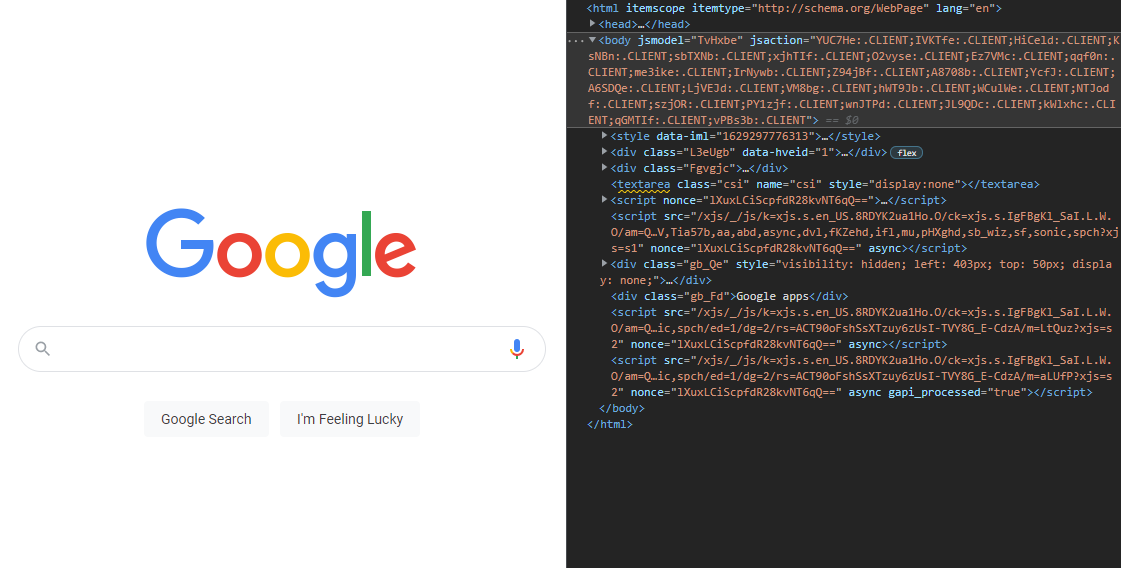
\includegraphics[width=0.8\linewidth]{google_html.png}
      \caption{Example -- HTML for websites}
      \label{fig:html}
    \end{figure}
  \end{frame}

  \begin{frame}{What is \LaTeX?}
    \LaTeX -- Markup language for academic documents (e.g., publications, presentations, lecture notes, assignments).
    \begin{figure}
      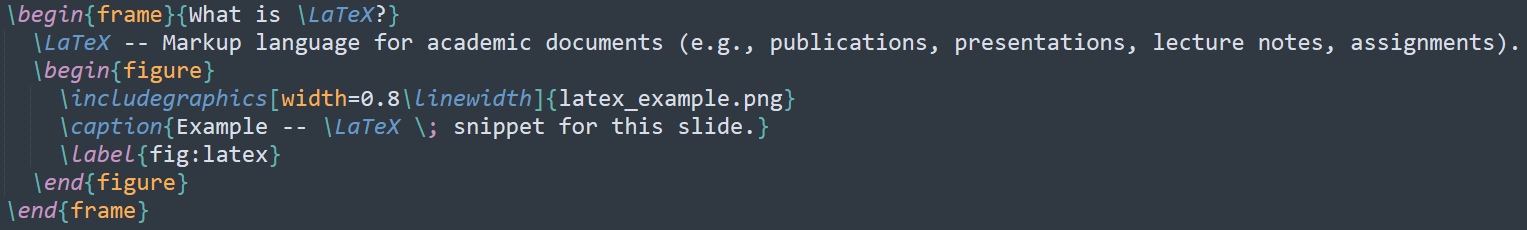
\includegraphics[width=0.8\linewidth]{latex_example.png}
      \caption{Example -- \LaTeX{}  snippet for this slide.}
      \label{fig:latex}
    \end{figure}
  \end{frame}


  % show some examples
  % equations, cross-references, citations, figures, and tables of contents
  \begin{frame}{Equations in \LaTeX}
    \begin{equation}
      V_s = \int_{-R}^R \pi (R^2 - x^2) dx = \frac{4}{3}\pi R^3 \label{eq:sphere}
    \end{equation}
    \begin{figure}
      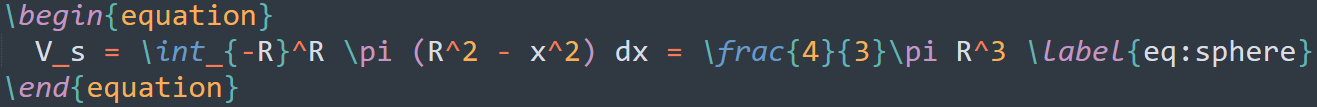
\includegraphics[width=0.8\linewidth]{equation_example.png}
      \caption{Example -- \LaTeX{} snippet for this equation.}
      \label{fig:equation}
    \end{figure}
  \end{frame}

  \begin{frame}{Cross-references in \LaTeX}
    Enables rich cross-referencing of equations, figures, tables
    \begin{itemize}
      \item Equation \ref{eq:sphere} (previous page)
      \item Table \ref{tab:ex-table} 
    \end{itemize}
    \begin{table}
      \centering
      \begin{tabular}{c|c}
        \textbf{Feature} & \textbf{Support} \\ \hline
        Figures & Yes! \\ \hline
        Equations & Yes! \\ \hline
        Tables & Yes! \\ \hline
        Bibliographies & Yes! \\ 
      \end{tabular}
      \caption{A simple table.}
      \label{tab:ex-table}
    \end{table}
  \end{frame}

  \begin{frame}{How does \LaTeX work?}
    Two primary components/steps:
    \begin{enumerate}
      \item Write your \LaTeX file(s) (\textbf{Text editor})
      \item ``Compile'' or ``Typeset'' your document (\textbf{\LaTeX \;system})
    \end{enumerate}
    \vspace{0.125in}
    \begin{figure}
      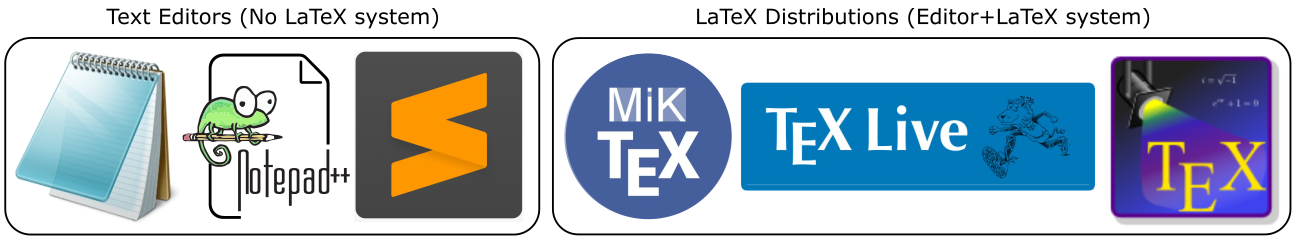
\includegraphics[width=0.8\linewidth]{tex_systems.png}
      \caption{Text editors (Notepad, Notepad++, Sublime Text) and LaTeX distributions (MikTeX, TeXLive, and TeX Studio)}
      \label{fig:systems}
    \end{figure}
  \end{frame}

  \begin{frame}{\LaTeX\;in this course}
    \begin{itemize}
      \item Editors/systems installed on local device (faster, private)
      \pause
      \item Editor/systems online (convenient, collaborative)
      \pause
      \item Will use \textbf{Overleaf} for this course (free account required)
    \end{itemize}
    \begin{figure}
      
\includegraphics[width=0.6\linewidth]{overleaf.png}
    \end{figure}
  \end{frame}

  \begin{frame}{Our First \LaTeX\;Project}
  \begin{enumerate}
    \item Make an Overleaf account (free!)
    \item Go to \texttt{https://www.overleaf.com/project}
    \item Create a blank project and pick a project name
  \end{enumerate}
    \begin{figure}
      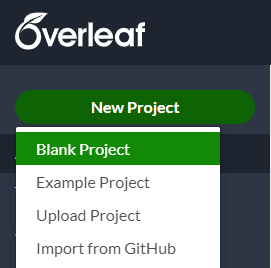
\includegraphics[width=0.3\linewidth]{day01-overleaf-00.png}
    \end{figure}
  \end{frame}

  \begin{frame}{Our First \LaTeX\;Project}
    \begin{figure}
      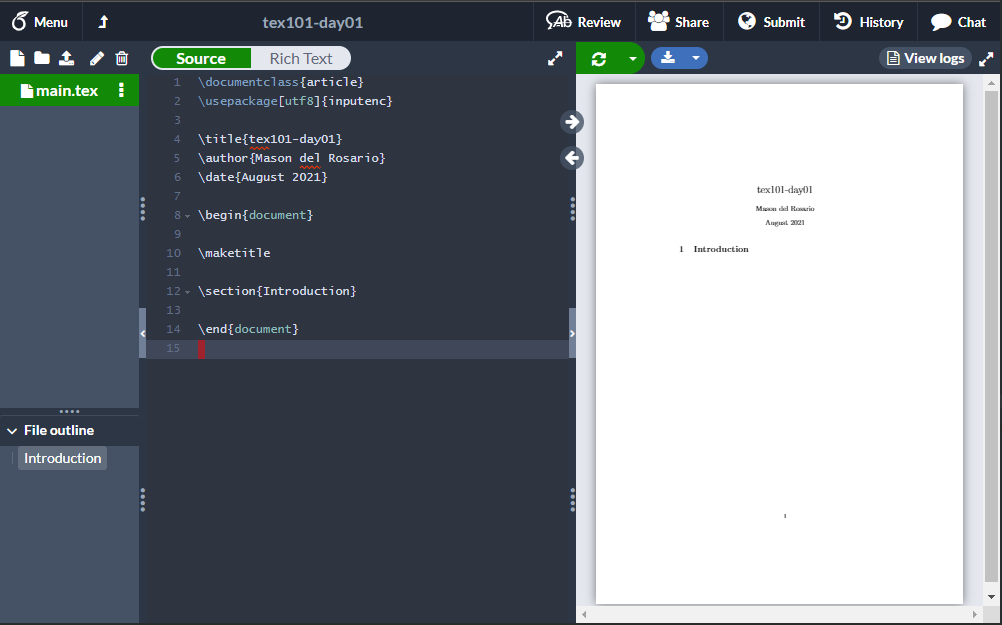
\includegraphics[width=0.9\linewidth]{day01-overleaf-01.png}
      \caption{Result of creating new project on Overleaf}
      \label{fig:day01-overleaf-01}
    \end{figure}
  \end{frame}

  \section{Document Structure}

  % Document structure section frame 
  \begin{frame}[plain]
    \vfill
    \centering
    \begin{beamercolorbox}[sep=8pt,center,shadow=true,rounded=true]{Document Structure}
      \usebeamerfont{title}\insertsectionhead\par%
      \color{davisblue}\noindent\rule{10cm}{1pt} \\
      \footnotesize{Commands, Environments, Errors}
    \end{beamercolorbox}
    \vfill
  \end{frame}

  \begin{frame}{Commands/Arguments}
    \LaTeX\;has special characters to define \underline{commands} and \underline{arguments}.
    \begin{itemize}
      \item Backslashes (\texttt{\textbackslash}) = start of a commands
      \item Curly brackets (\texttt{\{\}}) = mandatory arguments (i.e., inputs to commands)
      \item Square brackets (\texttt{[]}) = optional arguments
    \end{itemize}
  \end{frame}

  \nofoot{
  \begin{frame}{Backslashes/Commands}
    \begin{figure}
      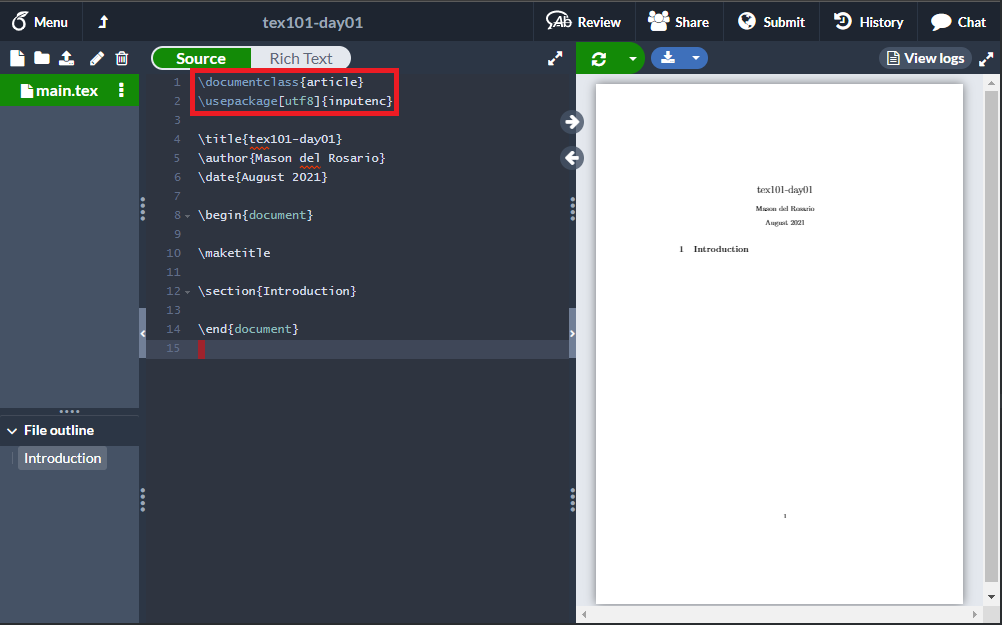
\includegraphics[width=0.9\linewidth]{day01-overleaf-01-docenc.png}
      \caption{Commands/arguments defining the document class and text encoding of our project.}
      \label{fig:day01-overleaf-01-docenc}
    \end{figure}
  \end{frame}
  }

  \nofoot{
  \begin{frame}{Backslashes/Commands}
    \begin{figure}
      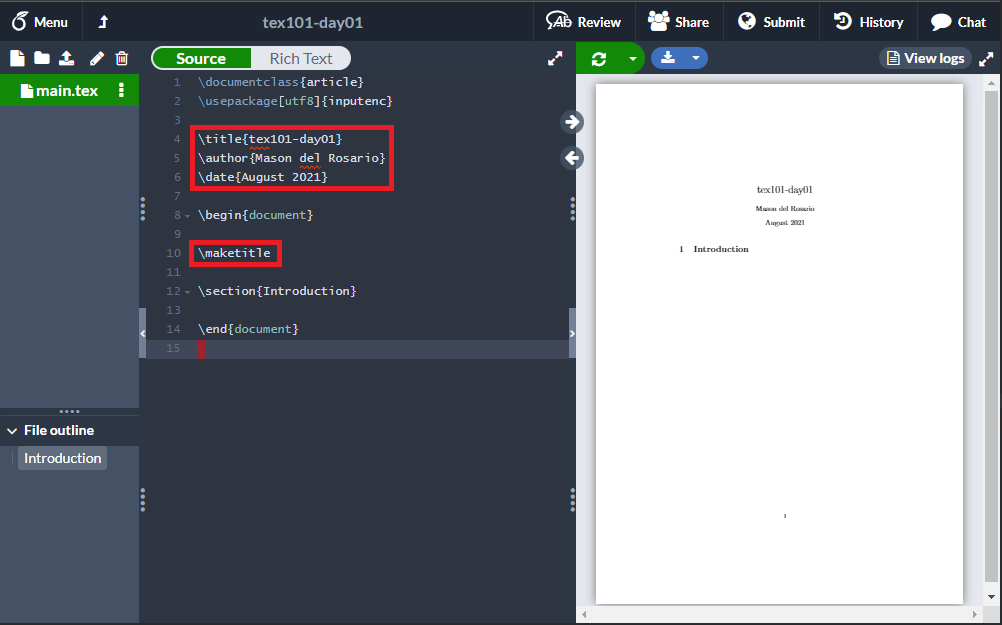
\includegraphics[width=0.9\linewidth]{day01-overleaf-01-title.png}
      \caption{Commands/arguments defining the title in our project.}
      \label{fig:day01-overleaf-01-title}
    \end{figure}
  \end{frame}
  }

  \nofoot{
  \begin{frame}{Environments}
    Environments = \texttt{\textbackslash begin\{...\}} and \texttt{\textbackslash end\{...\}} commands.
    \begin{figure}
      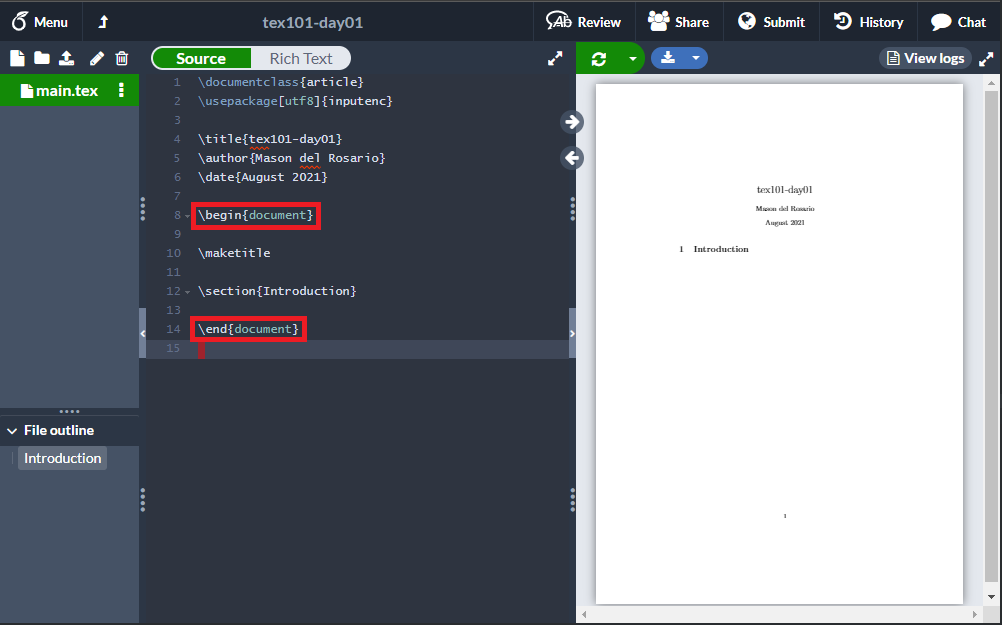
\includegraphics[width=0.9\linewidth]{day01-overleaf-02.png}
      \caption{Every \LaTeX\;file includes a \texttt{document} environment.}
      \label{fig:day01-overleaf-02}
    \end{figure}
  \end{frame}
  }

  % equation
  \nofoot{
  \begin{frame}{Environments}
    Lots of different environments! Will go over more in this course.
    \begin{figure}
      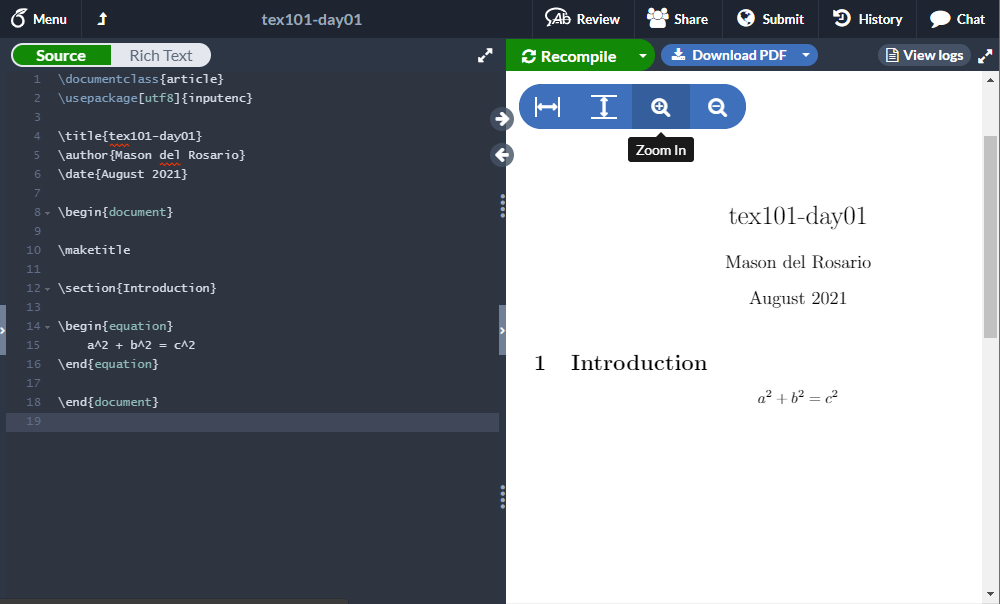
\includegraphics[width=0.9\linewidth]{day01-overleaf-03.png}
      \caption{Try writing an \texttt{equation} environment!}
      \label{fig:day01-overleaf-02}
    \end{figure}
  \end{frame}
  }

  % error - remove command to produce the error
  \nofoot{
  \begin{frame}{Errors}
    \begin{itemize}
      \item What happens when we mess up?
      \item Remove the \texttt{\textbackslash end\{equation\}} command, compile the document.
    \end{itemize}
    \pause 
    \begin{figure}
      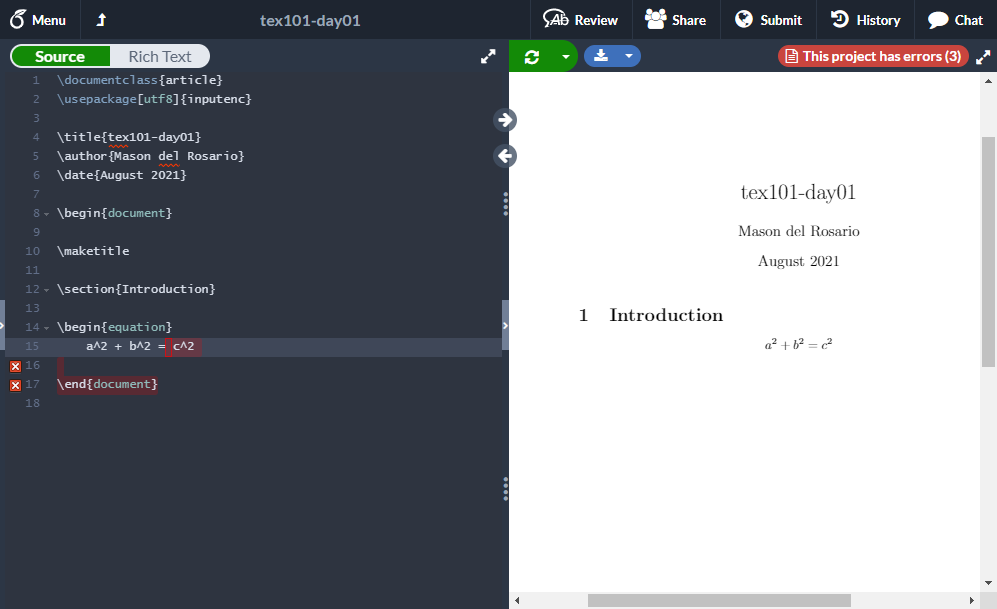
\includegraphics[width=0.9\linewidth]{day01-overleaf-04-remove.png}
      \caption{Click on the \textcolor{red}{red badge} to reveal more details.}
      \label{fig:day01-overleaf-04-remove}
    \end{figure}
  \end{frame}
  }

  % error - details
  \nofoot{
  \begin{frame}{Errors}
    Some errors might be sneakier. Google is your friend!
    \begin{figure}
      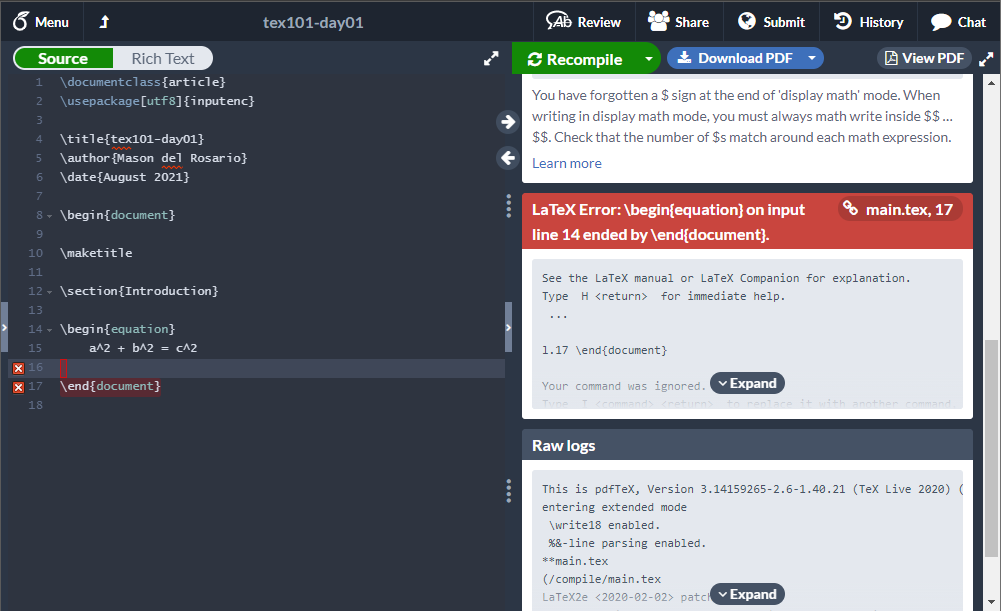
\includegraphics[width=0.9\linewidth]{day01-overleaf-04-error.png}
      \caption{Compiler has returned an \textcolor{red}{error}.}
      \label{fig:day01-overleaf-04-error}
    \end{figure}
  \end{frame}
  }

  \begin{frame}{Exercise: Text and Whitespace}
    \begin{itemize}
      \item Try adding text to your project, recompiling, and seeing the changes in your PDF.
      \item Add some paragraphs with variable spacing. How does \LaTeX{} handle multiple spaces?
      % \item Explore how your editor works; double click somewhere on your PDF, and see where your cursor moves in your source file.
      \item Share your observations/questions in chat!
    \end{itemize}
  \end{frame}

  \section{Logical structure}

  % Logical structure section frame 
  \begin{frame}[plain]
    \vfill
    \centering
    \begin{beamercolorbox}[sep=8pt,center,shadow=true,rounded=true]{Background}
      \usebeamerfont{title}\insertsectionhead\par%
      \color{davisblue}\noindent\rule{10cm}{1pt} \\
      \footnotesize{Text formatting, sectioning, lists}
    \end{beamercolorbox}
    \vfill
  \end{frame}

  \begin{frame}{Text Formatting}
    Some common commands for formatting text:
    \begin{itemize}
      \item \texttt{\textbackslash textbf}: \textbf{Make text boldface.}
      \item \texttt{\textbackslash textit}: \textit{Make text italic.}
      \item \texttt{\textbackslash underline}: \underline{Underline text.}
      \item \texttt{\textbackslash texttt}: \texttt{Make text resemble typewriter.}
      \item And so many more! For example, see \texttt{https://latex-tutorial.com/changing-font-style/}.
    \end{itemize}
  \end{frame}

  \begin{frame}{Sectioning commands}
    \LaTeX\; provides commands to generate section/subsection headings. 
    \begin{figure}
      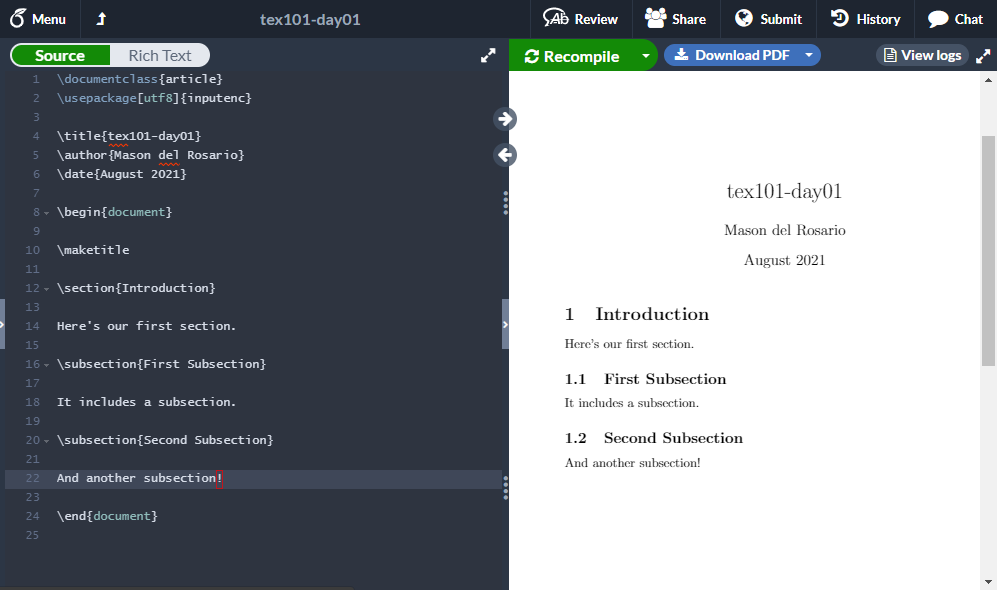
\includegraphics[width=0.9\linewidth]{day01-overleaf-05-sections.png}
      \caption{Numbers for different (sub)sections are automatically generated.}
      \label{fig:day01-overleaf-05-sections}
    \end{figure}
  \end{frame}

  \begin{frame}{Sectioning commands}
    Different section levels available:
    \begin{itemize}
      \item \texttt{\textbackslash chapter} (for \texttt{\textbackslash documentclass\{book\}}, \texttt{\textbackslash documentclass\{report\}})
      \item \texttt{\textbackslash section}
      \item \texttt{\textbackslash subsection}
      \item \texttt{\textbackslash subsubsection}
      \item \texttt{\textbackslash paragraph} (rarely used!)
    \end{itemize}
  \end{frame}

  \begin{frame}{Lists}
    \begin{multicols}{2}
    [\centering Lists in \LaTeX can be unordered or ordered:]
      \begin{itemize}
        \item First unordered item
        \item Second unordered item
        \item Third unordered item
      \end{itemize}
      \columnbreak
      \begin{enumerate}
        \item First ordered item
        \item Second ordered item
        \item Third ordered item
      \end{enumerate}
    \end{multicols}
  \end{frame}

  \begin{frame}{Lists}
    List commands: \texttt{itemize/enumerate} environments + \texttt{\textbackslash item} commands per each line.
    \begin{figure}
      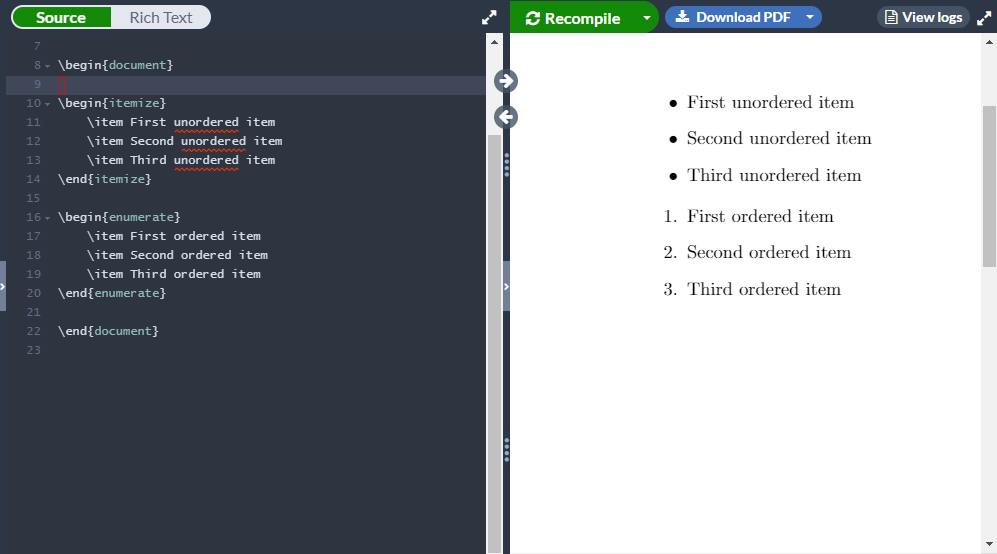
\includegraphics[width=0.9\linewidth]{day01-overleaf-06-lists.png}
      \caption{Numbers for different (sub)sections are automatically generated.}
      \label{fig:day01-overleaf-06-lists}
    \end{figure}
  \end{frame}

  \begin{frame}{Exercises}
  \begin{itemize}
    \item Try formatting some text. Can you find any new formats at \texttt{https://latex-tutorial.com/changing-font-style/}?
    % \item Experiment with different sectioning levels. Try using \texttt{\textbackslash documentclass\{report\}} instead of \texttt{\textbackslash documentclass\{article\}} and adding \texttt{\textbackslash chapter} commands. How do they look?
    \item Try out \texttt{\textbackslash paragraph} and \texttt{\textbackslash subparagraph} to see how they work (by default, they don’t add numbers).
    \item Make some lists, and nest one list inside another. How does the format of the numbers or markers change? (You can only go to four levels with standard \LaTeX.)
  \end{itemize}
  \end{frame}

  \section{Document Classes}
  % Logical structure section frame 

  \begin{frame}[plain]
    \vfill
    \centering
    \begin{beamercolorbox}[sep=8pt,center,shadow=true,rounded=true]{Document Classes}
      \usebeamerfont{title}\insertsectionhead\par%
      \color{davisblue}\noindent\rule{10cm}{1pt} \\
      \footnotesize{Base classes, presentations}
    \end{beamercolorbox}
    \vfill
  \end{frame}

  \begin{frame}{What \texttt{\textbackslash documentclass} does}
    Controls general layout of document, changing:
    \begin{itemize}
      \item Design (margins, fonts, spacing, etc.)
      \item Sectioning (e.g., \texttt{\textbackslash chapter})
      \item Title location (top of page vs. separate page)
      \item Add new commands (e.g., \texttt{frame} environments for slides)
    \end{itemize}
    \pause
    Can manually set global options (i.e., \texttt{\textbackslash documentclass[<options>]\{<name>\}}).
  \end{frame}
  
  \begin{frame}{Chapters}
    \begin{figure}
      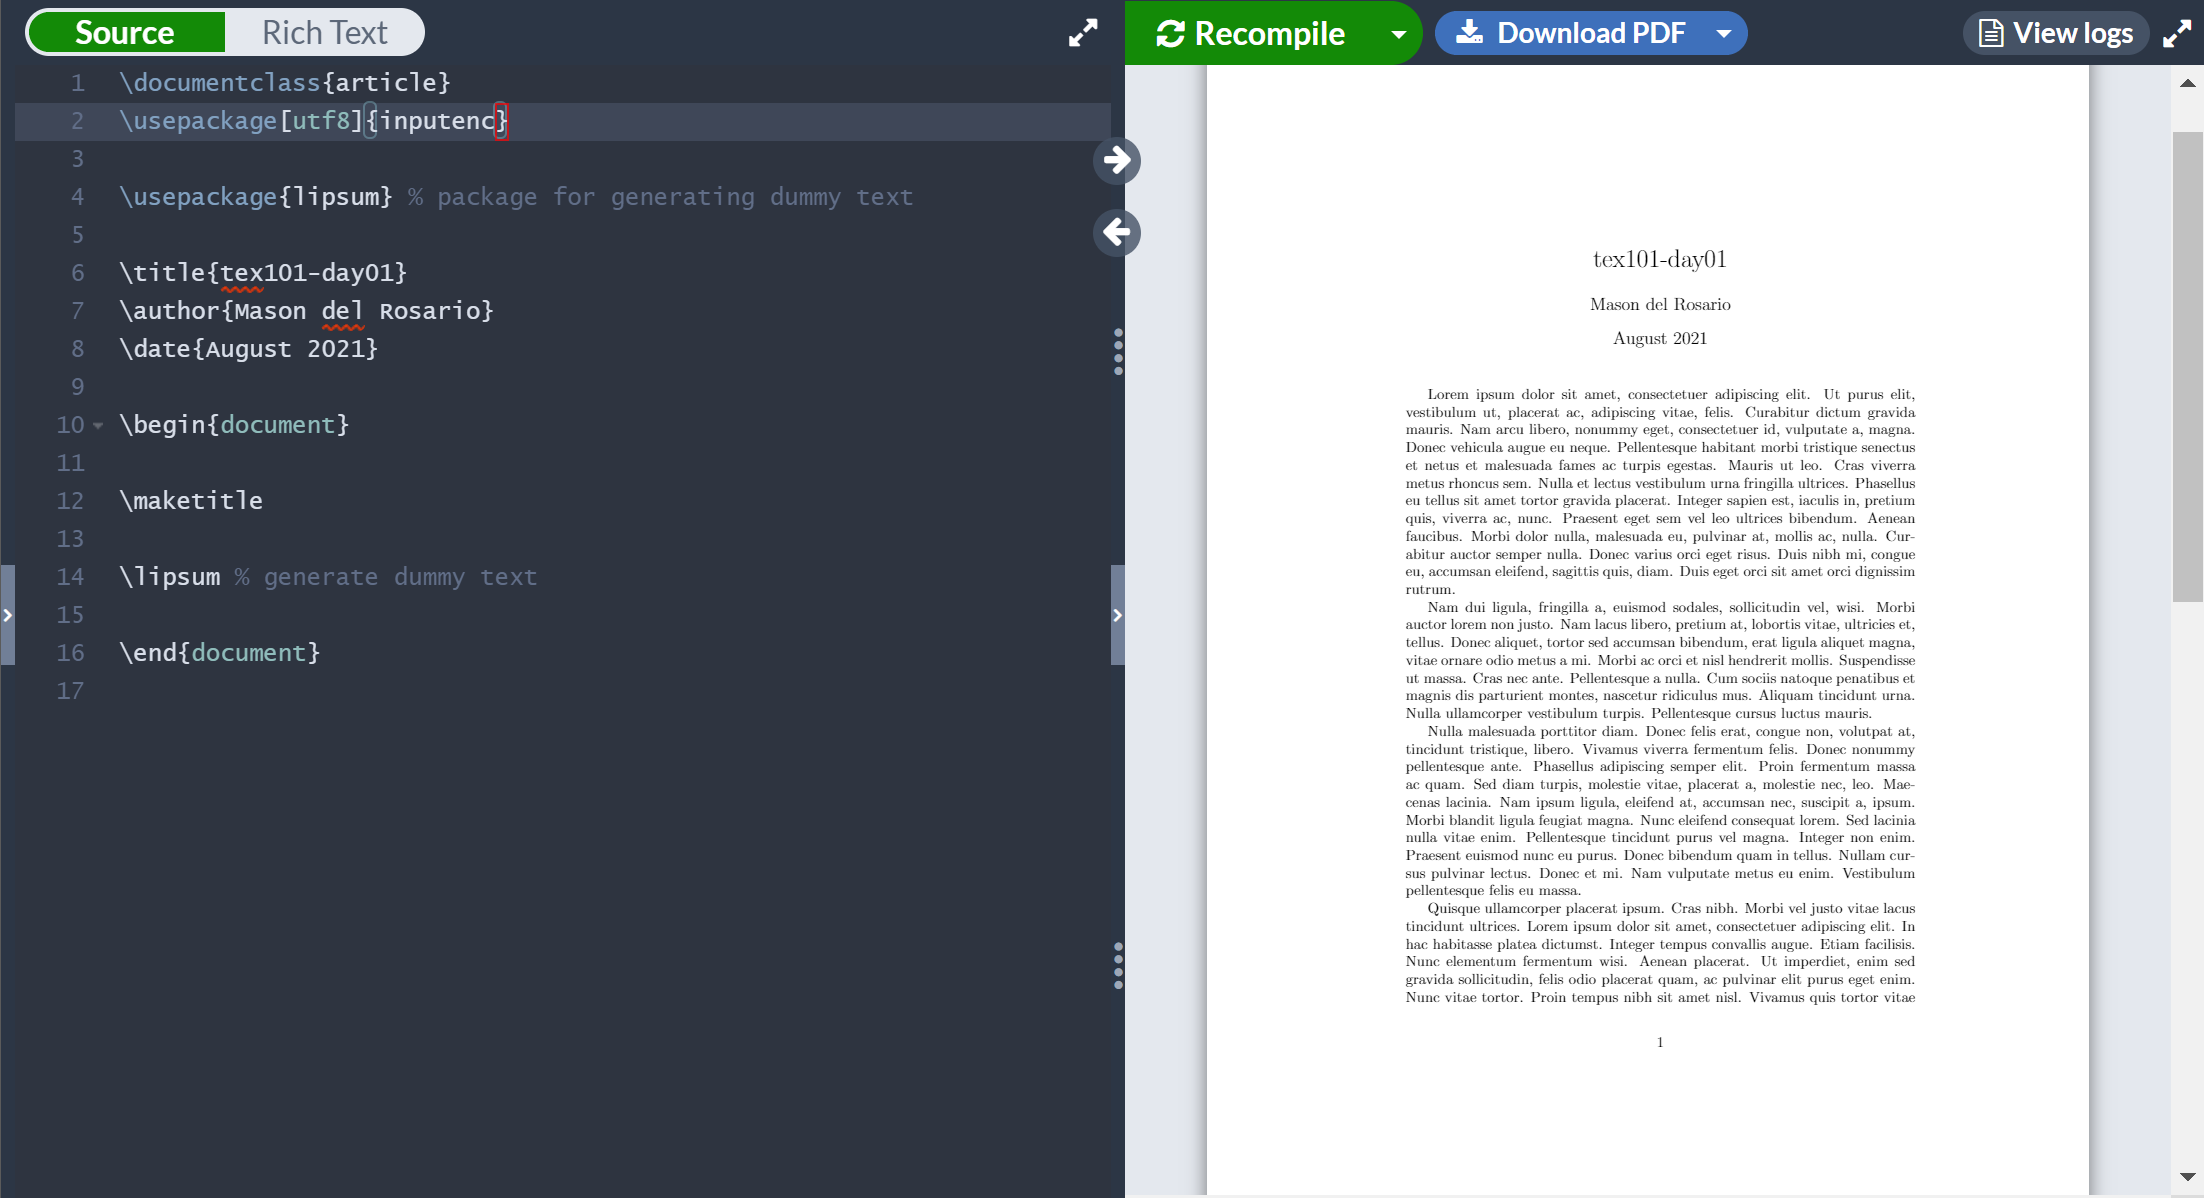
\includegraphics[width=0.9\linewidth]{day01-overleaf-07A-article.png}
      \caption{Our starter project is an \texttt{article} class.}
      \label{fig:day01-overleaf-07A}
    \end{figure}
  \end{frame}

  \begin{frame}{Chapters}
    \begin{figure}
      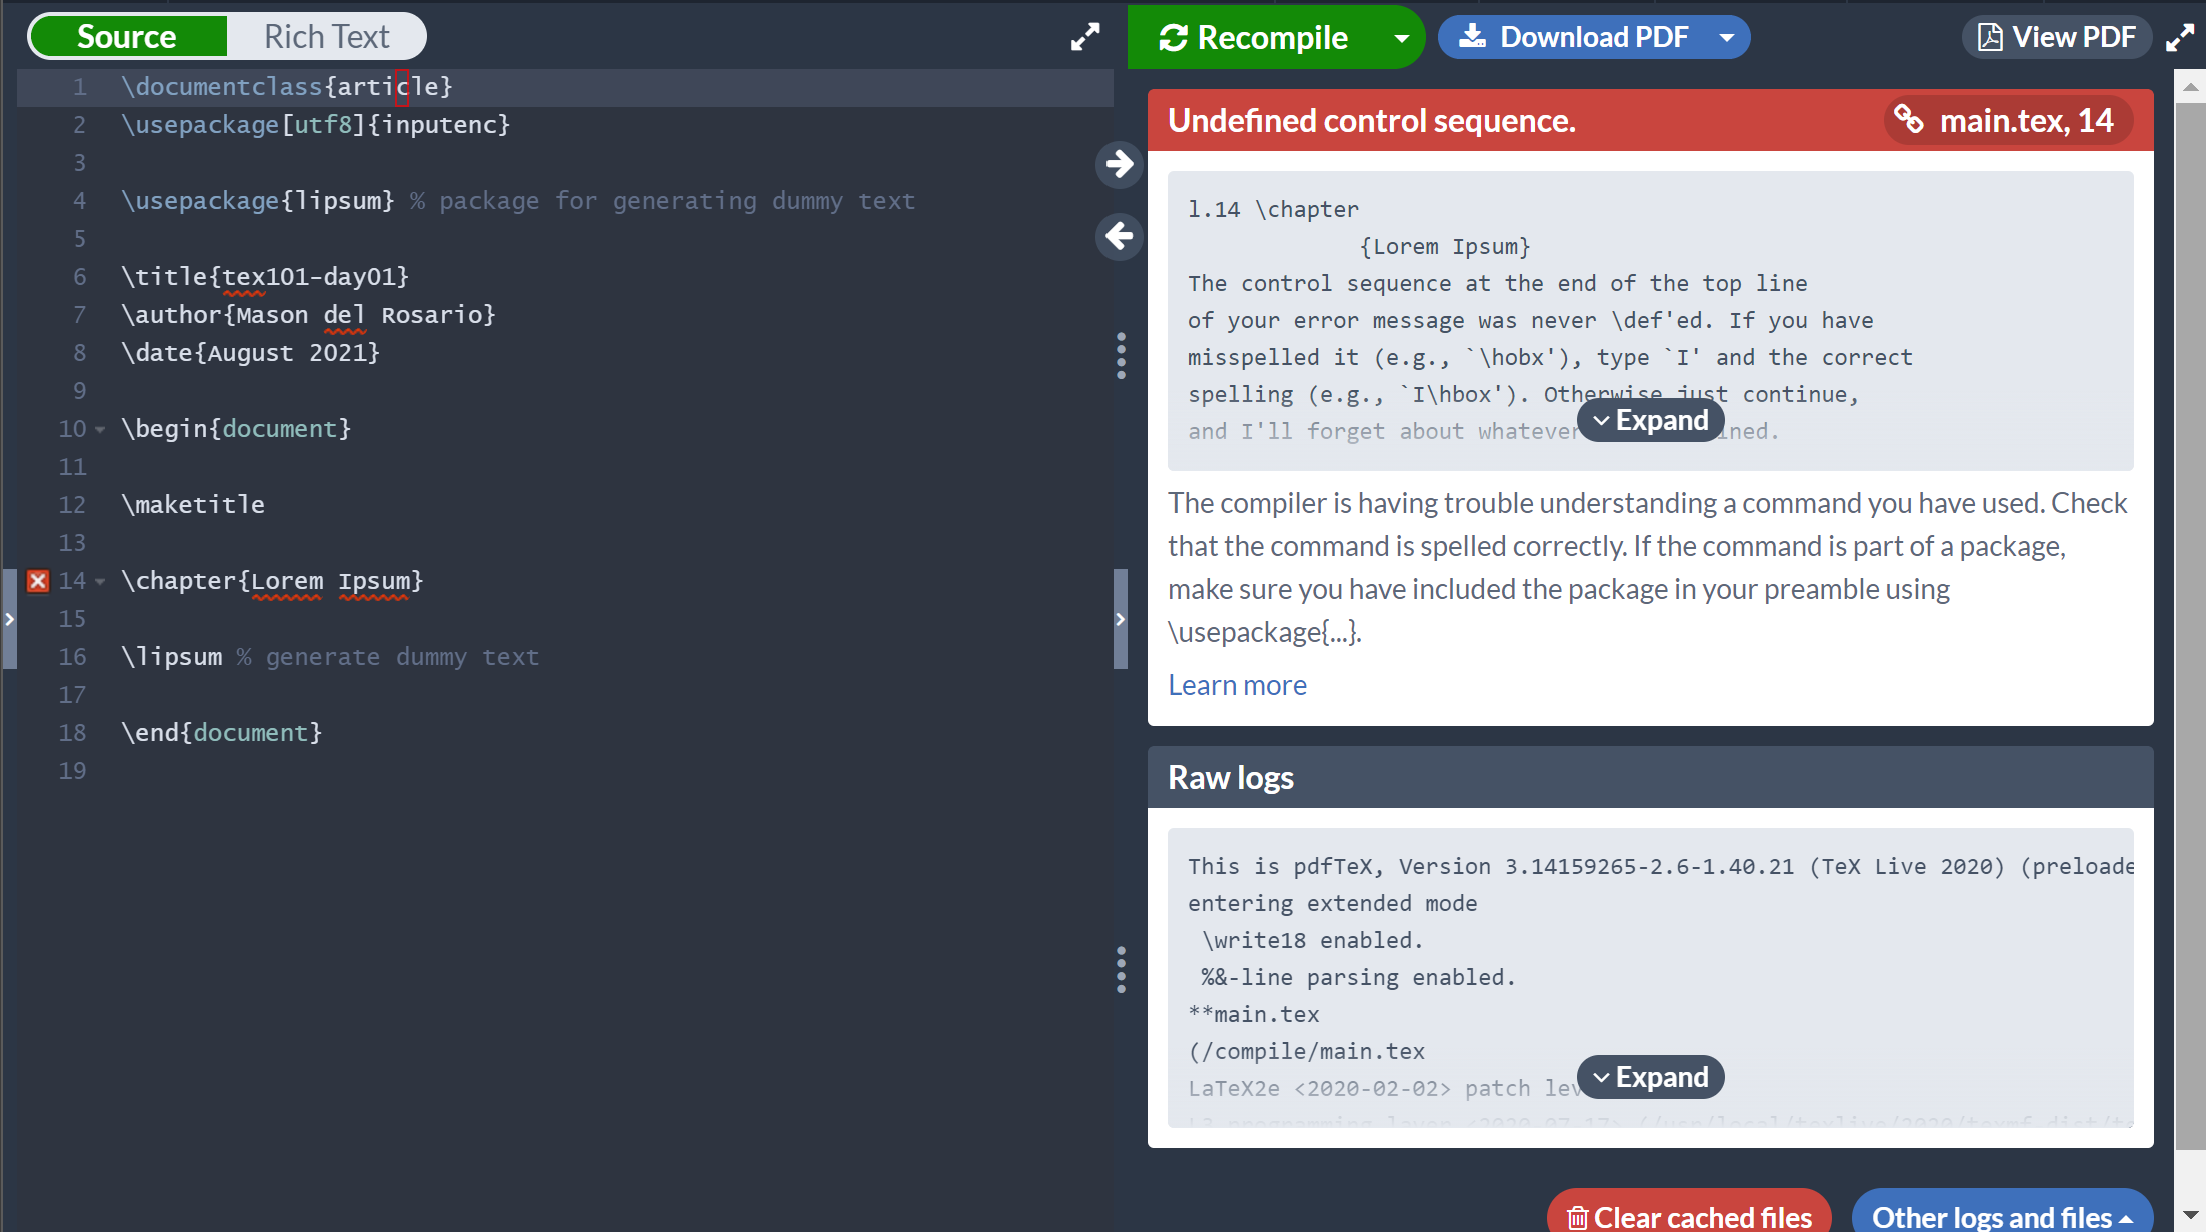
\includegraphics[width=0.9\linewidth]{day01-overleaf-07B-chapter-error.png}
      \caption{Adding a \texttt{\textbackslash chapter}  causes an error.}
      \label{fig:day01-overleaf-07B}
    \end{figure}
  \end{frame}

  \begin{frame}{Chapters}
    \begin{figure}
      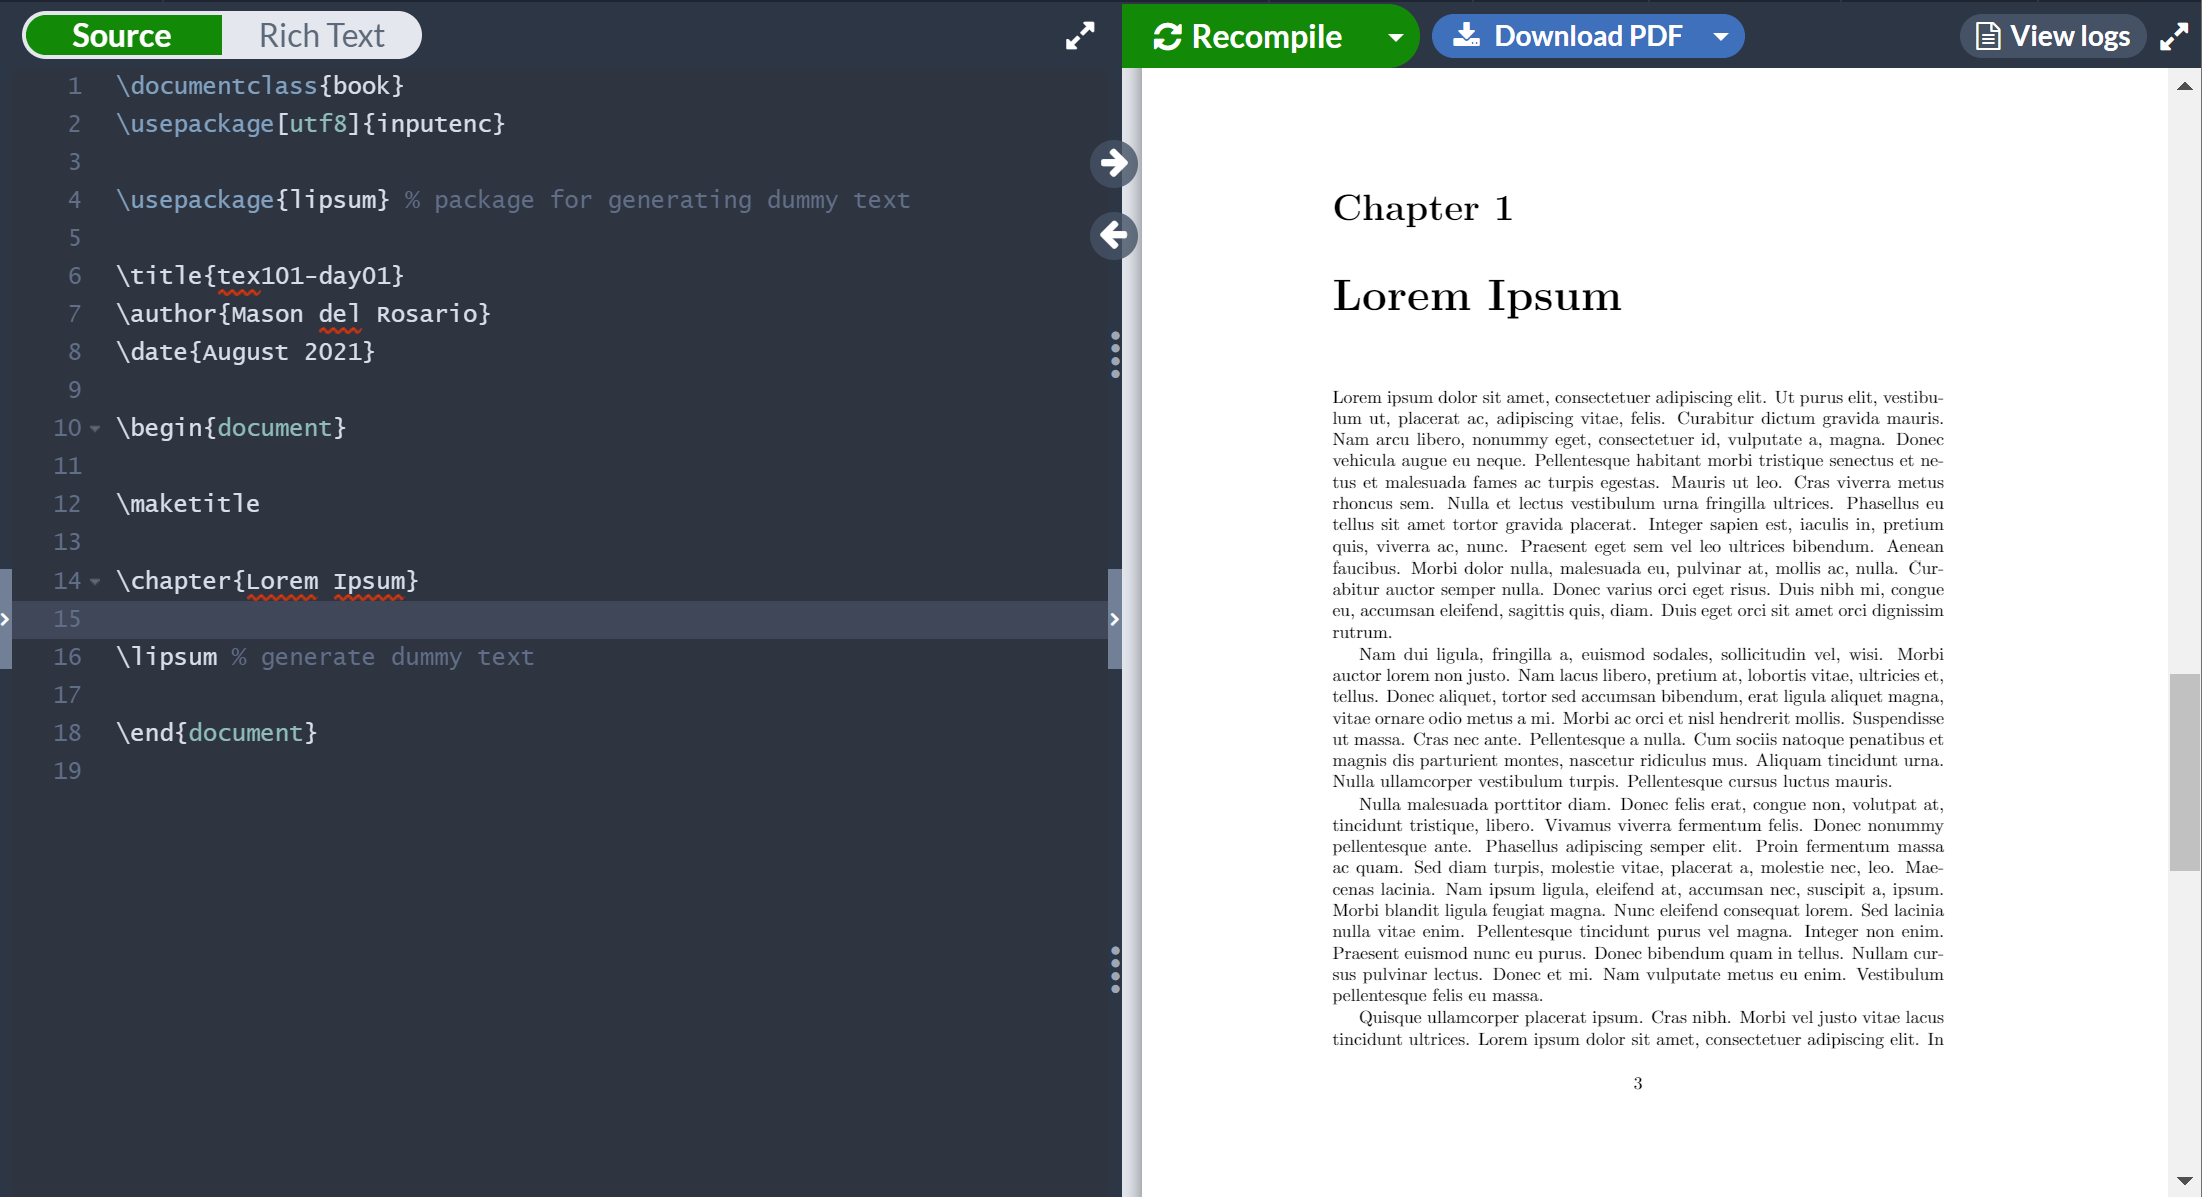
\includegraphics[width=0.9\linewidth]{day01-overleaf-07C-chapter-fix.png}
      \caption{Changing to \texttt{\textbackslash documentclass\{book\}} enables \texttt{\textbackslash chapter}.}
      \label{fig:day01-overleaf-07C}
    \end{figure}
  \end{frame}

  \begin{frame}{Base classes}
    Default \texttt{\textbackslash documentclass}es provided by \LaTeX:
    \begin{itemize}
      \item \texttt{article} - short documents without chapters
      \item \texttt{report} - longer documents with chapters, single-sided printing
      \item \texttt{book} - longer documents with chapters, double-sided printing, front-/back-matter (e.g., index)
      \item \texttt{letter} - correspondence with no sections
      \item \texttt{slides} - for presentations (not used in practice; will explain!)
    \end{itemize}
  \end{frame}

  \begin{frame}{Exercises}
    \begin{itemize}
      \item Explore changing the document class between base classes (e.g., \texttt{letter}, \texttt{report}). How do these affect the appearance of the document?
      \item Using the square brackets (\texttt{[]}), add the option \texttt{twocolumn} to your \texttt{documentclass}. How does this affect the layout of the document?
    \end{itemize}
  \end{frame}

  \section{Packages and Definitions}
  % Packages and definitions 

  \begin{frame}[plain]
    \vfill
    \centering
    \begin{beamercolorbox}[sep=8pt,center,shadow=true,rounded=true]{Extending LaTeX}
      \usebeamerfont{title}\insertsectionhead\par%
      \color{davisblue}\noindent\rule{10cm}{1pt} \\
      \footnotesize{Packages and definitions}
    \end{beamercolorbox}
    \vfill
  \end{frame}

  \begin{frame}{Packages}
    Base \LaTeX doesn't do everything. \underline{Packages} add more functionality, including:
    \begin{itemize}
      \item Change how parts of \LaTeX work
      \item Add new commands (e.g. \texttt{\textbackslash lipsum} package for filler text)
      \item Change document design
    \end{itemize}
  \end{frame}


  % \begin{frame}{Packages}
  %   \textbf{Example: \texttt{babel}} -- rule sets for different languages.%\footnote[]More here: \url{https://www.learnlatex.org/en/more-06#the-babel-package}
  %   \begin{figure}
  %     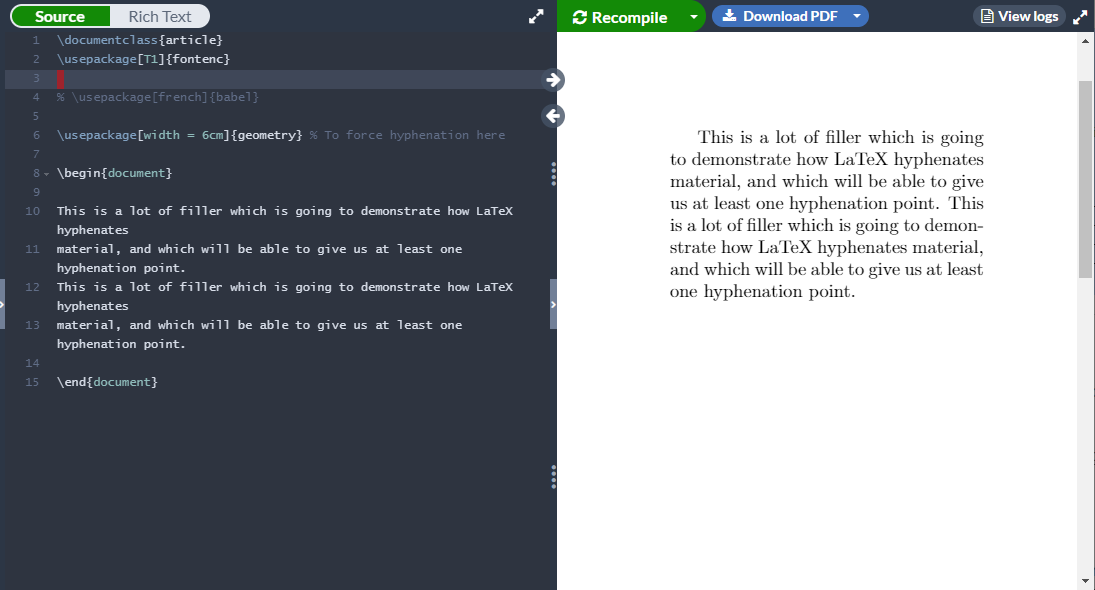
\includegraphics[width=0.9\linewidth]{day01-overleaf-08A-package-geom.png}
  %     \caption{Filler text without using \texttt{babel} package.}
  %     \label{fig:day01-overleaf-08A}
  %   \end{figure}
  % \end{frame}

  % \begin{frame}{Packages}
  %   \textbf{Example: \texttt{babel}} -- rule sets for different languages.%\footnote[]More here: \url{https://www.learnlatex.org/en/more-06#the-babel-package}
  %   \begin{figure}
  %     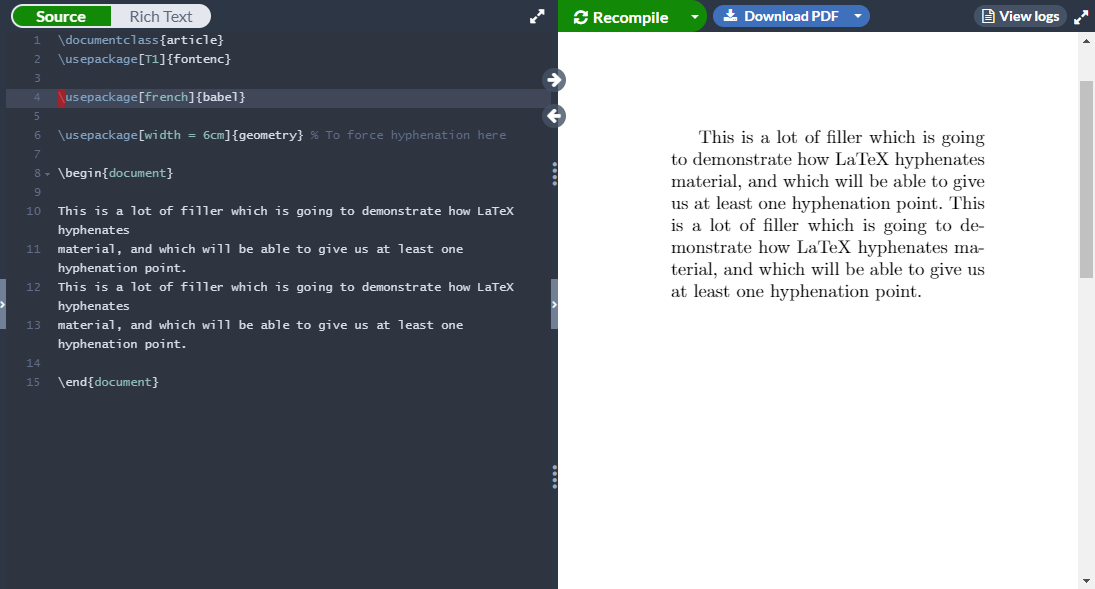
\includegraphics[width=0.9\linewidth]{day01-overleaf-08B-package-babel.png}
  %     \caption{\texttt{babel} package with french option changes hyphenation.}
  %     \label{fig:day01-overleaf-08B}
  %   \end{figure}
  %   % \footnotetext[1]{More here: \url{https://www.learnlatex.org/en/more-06#the-babel-package}}    
  % \end{frame}

  \begin{frame}{Packages}
    \textbf{Example: \texttt{geometry}} -- enables direct control of margins, borders, line spacing, etc.
    \begin{figure}
      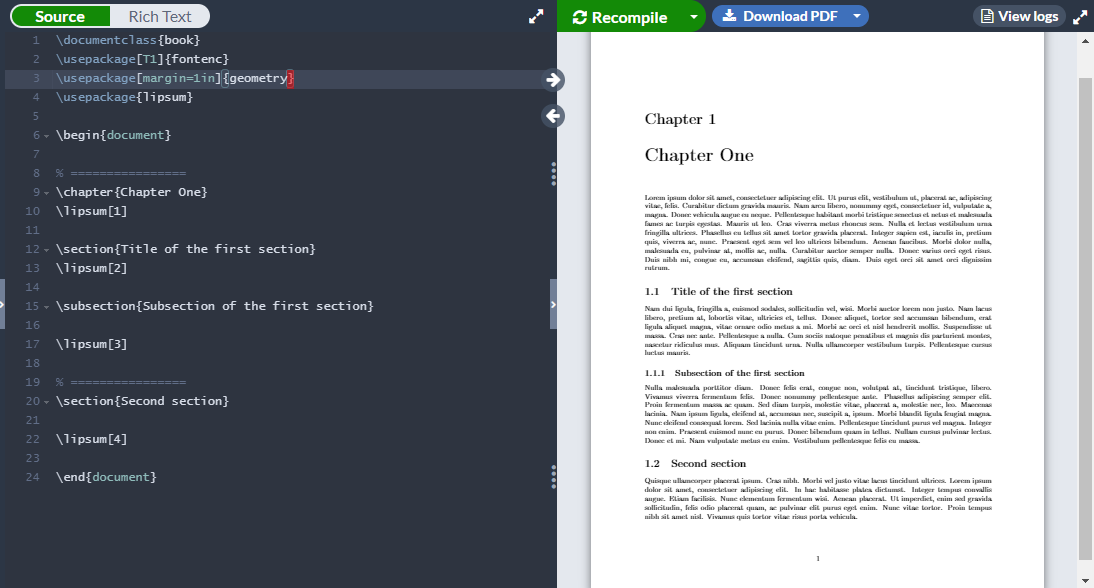
\includegraphics[width=0.9\linewidth]{day01-overleaf-08C-package-geom-redux.png}
      \caption{\texttt{geometry} package with 1" page margins.}
      \label{fig:day01-overleaf-08C}
    \end{figure}
  \end{frame}

  \begin{frame}{Packages}
    \textbf{Example: \texttt{geometry}} -- enables direct control of margins, borders, line spacing, etc.
    \begin{figure}
      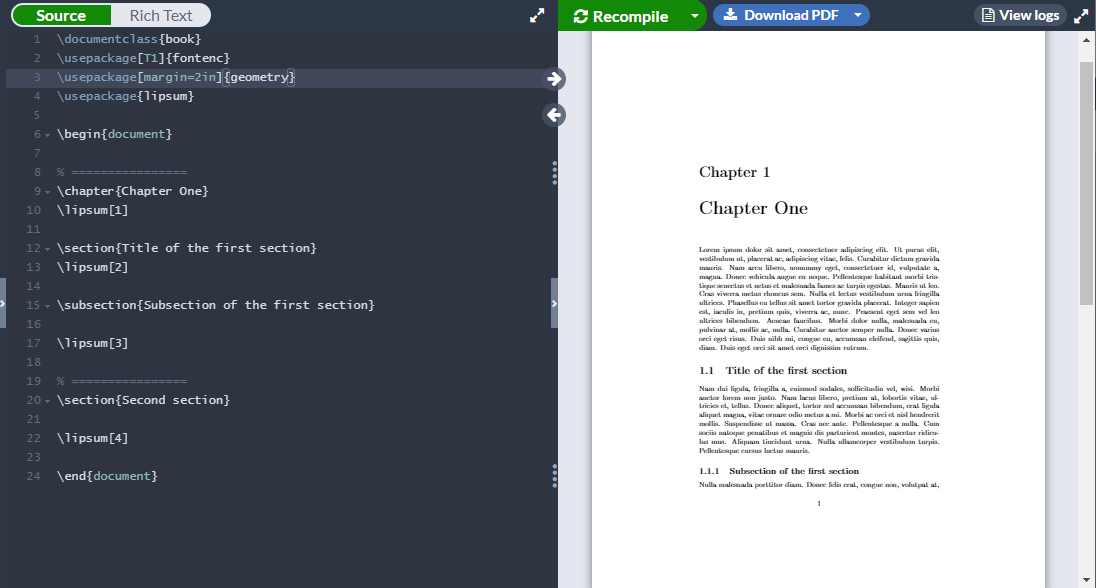
\includegraphics[width=0.9\linewidth]{day01-overleaf-08D-package-geom-redux.png}
      \caption{\texttt{geometry} package with 2" page margins.}
      \label{fig:day01-overleaf-08D}
    \end{figure}
  \end{frame}

  \begin{frame}{Definitions}
    Can't find a command you want? Want to avoid repeating yourself? 

    Use definitions to define your own commands!
  \end{frame}

  \begin{frame}{Definitions}
    Line 6 \texttt{\textbackslash newcommand} defines a \texttt{\textbackslash kw} command.
    \begin{itemize}
      \item \texttt{\textbackslash newcommand\textbackslash kw} $\to$ assign \texttt{kw} as command name
      \item \texttt{[1]} $\to$ number of arguments
      \item \texttt{\#1} $\to$ first argument supplied to command
    \end{itemize}
    \begin{figure}
      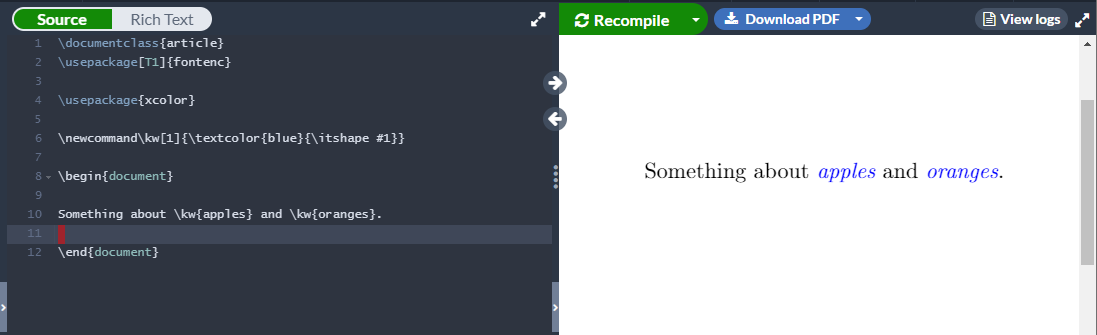
\includegraphics[width=0.9\linewidth]{day01-overleaf-09A-defn.png}
      \caption{A definition for a custom `keyword' command \texttt{\textbackslash kw}.}
      \label{fig:day01-overleaf-09A}
    \end{figure}
  \end{frame}

  \begin{frame}{Day 01 Summary}
    Today we covered:
    \begin{itemize}
      \item Document structure (commands, environments, errors)
      \item Logical structure (sections, environments, lists)
      \item Document classes (base classes)
      \item Packages and definitions
    \end{itemize}
  \end{frame}

  \begin{frame}{Day 01 Break Time}
    When we come back, I'll introduce the exercise:
    \begin{itemize}
      \item \href{https://github.com/mdelrosa/latex101/blob/master/day01/exercise/day-01-exercise.pdf}{Day 01 Exercise (Github)}
    \end{itemize}
  \end{frame}

\begin{frame}{End of Day 01}
  \begin{itemize}
    \item Finished Lessons 1-6 from \texttt{learnlatex.org}
    \item Tomorrow: Lessons 7-12 from \texttt{learnlatex.org}
    \item Questions? Ask on the Slack channel! (\#latex101)
  \end{itemize}
\end{frame}

} %end footnotsize

\end{document}
